\section{Massless Vector Exchange\label{SecMasslessVec4}}
%%%%%%%%%%%%%%%%%%%%%%%%%%%%%%%%%%%%%%%%%%%%%%%%%%%%%%%%%%%%%%%%%%%%%%%%%%%%%%%%%%%%%%%%%
We now start with a two-boy path integral for scalar particles coupled to an external vector field $A_{m}$:
\begin{equation}
	\mathcal{G}_{A}[A] = \int\limits_{x_{1}}^{x_{3}} \mathrm{D}q_{a}(\tau) \int\limits_{x_{2}}^{x_{4}} \mathrm{D}q_{b}(\sigma) \, \exp{\left(- i S_{0}[q_{a}, q_{b}] - i S_{\text{int}}[q_{a}, q_{b}, A] \right)}
\end{equation}
The free term $S_{0}$ is given by (\ref{FreeS}) and the interaction term is
\begin{equation}
	S_{\text{int}}[q_{a}, q_{b}, A] \equiv Z_{a} \int \mathrm{d}\tau \left( \dot{q}_{a} \cdot A[q_{a}(\tau)] \right) + Z_{b} \int \mathrm{d}\sigma \left( \dot{q}_{b} \cdot A[q_{b}(\sigma)] \right) \label{SintVec}
\end{equation}
Here $Z_{a}$ and $Z_{b}$ are the dimensionless (electric) charges of particles $a$ and $b$.

We integrate over the field $A_{m}$ to obtain the ``effective'' interacting two-body path integral:
\begin{equation}
	\mathcal{F}_{A} \equiv \int \mathrm{D}A_{m}(x) \, \mathcal{G}_{A}[A] \exp{\left( -i S_{\text{kin}}[A] \right)}
\end{equation}
where $S_{\text{kin}}$ contains the gauge-fixed kinetic operator,
\begin{equation}
	S_{\text{kin}}[A] = \frac{1}{2g_{1}^{2}} \int \int \mathrm{d}x \mathrm{d}y \left[ A_{m}(x) (K_{1})^{mn}(x|y) A_{n}(y) \right] \label{SkinVec}
\end{equation}
with
\begin{equation}
	(K_{1})^{mn}(x|y) \equiv \delta(x - y) \left[-\frac{1}{2}\eta^{mn}\partial^{2} + \frac{1}{2} \left(1 - \frac{1}{\xi_{1}} \right) \partial^{m} \partial^{n} \right]
\end{equation}
In the Fermi-Feynman gauge ($\xi_{1} = 1$) we have
\begin{equation}
	(K_{1})^{mn}(x|y) = \eta^{mn} K_{0}(x|y)
\end{equation}
where $K_{0}$ is the massless scalar kinetic operator. We rewrite $S_{\text{int}}$ as
\begin{equation}
	S_{\text{int}}[q_{a}, q_{b}, A] = \int \mathrm{d}x \, J^{m}(x) A_{m}(x)
\end{equation}
with
\begin{equation}
	J^{m}(x) \equiv Z_{a} \int \mathrm{d}\tau \, \dot{q}_{a}^{m} \delta[x - q_{a}(\tau)] + Z_{b} \int \mathrm{d}\sigma \, \dot{q}_{b}^{m} \delta[x - q_{b}(\sigma)]
\end{equation}
After integrating over $A_{m}$, we find
\begin{equation}
	\mathcal{F}_{A} = \int\limits_{x_{1}}^{x_{3}} \mathrm{D}q_{a}(\tau) \int\limits_{x_{2}}^{x_{4}} \mathrm{D}q_{b}(\sigma) \, \exp{\left(- i S_{A}[q_{a}, q_{b}] \right)}
\end{equation}
where
\begin{equation}
	S_{A}[q_{a}, q_{b}] \equiv S_{0}[q_{a}, q_{b}] - \frac{g_{1}^{2}}{2} \int \int \mathrm{d} x \mathrm{d} y \left[ J^{m}(x) (G_{1})_{mn}(x|y) J^{n}(y) \right]
\end{equation}
In analogy with (\ref{JGJSca}) we can use the explicit form of $J^{m}$ to write
\begin{equation}
	\frac{g_{1}^{2}}{2} \int \int \mathrm{d} x \mathrm{d} y \left[ J^{m}(x) (G_{1})_{mn}(x|y) J^{n}(y) \right] = S_{1}^{A}[q_{a}, q_{b}] + S_{2}^{A}[q_{a}, q_{b}]
\end{equation}
with $S_{1}^{A}$ containing self-interactions,
\begin{equation}
\begin{split}
	S_{1}^{A}[q_{a}, q_{b}] = {}& \frac{Z_{a}^{2} g_{1}^{2}}{2} \int \int \mathrm{d}\tau_{1} \mathrm{d}\tau_{2} \left[ \dot{q}_{a}(\tau_{1}) \cdot \dot{q}_{a}(\tau_{2}) \right] G_{0}[q_{a}(\tau_{1}) | q_{a}(\tau_{2})] \\
	&+ \frac{Z_{b}^{2}g_{1}^{2}}{2} \int \int \mathrm{d}\sigma_{1} \mathrm{d}\sigma_{2} \left[ \dot{q}_{b}(\sigma_{1}) \cdot \dot{q}_{b}(\sigma_{2}) \right] G_{0}[q_{b}(\sigma_{1}) | q_{b}(\sigma_{2})]
\end{split}
\end{equation}
and $S_{2}^{A}$ containing two-body interactions,
\begin{equation}
	S_{2}^{A}[q_{a}, q_{b}] = Z_{a} Z_{b} g_{1}^{2} \int \int \mathrm{d}\tau \mathrm{d}\sigma \left[ \dot{q}_{a}(\tau) \cdot \dot{q}_{b}(\sigma) \right] G_{0}\left[ q_{a}(\tau) | q_{b}(\sigma) \right] \label{S2Vec}
\end{equation}
Just like in the previous section, we will \textit{ignore} the contributions from $S_{1}^{A}$.

As we found in section \ref{SecDimAn}, the coupling parameter $g_{1}$ has units
\begin{equation}
	[g_{1}] = \left( \frac{4 - D}{2} \right) [\text{mass}]
\end{equation}
In $D = 4$, we have that $g_{1}$ is dimensionless. We write
\begin{equation}
	g_{1}^{2} = \frac{\alpha_{1}}{2 \pi} \mu^{(4 - D)}
\end{equation}
where $\mu$ has units of mass, and $\alpha_{1}$ is dimensionless. Similarly, in $D = 3$ we have that $g_{1}^{2}$ has units of mass. Thus, we write
\begin{equation}
	g_{1}^{2} = \frac{\beta_{1}}{(2 \pi)^{3/2}} \mu^{(3 - D)}
\end{equation}
where $\mu$ and $\beta_{1}$ have units of mass.
%Unlike in the previous chapter, we find that $g_{1}$ has the expected mass-dimension for a coupling parametrizing the interaction of matter with vector quanta. However, the field $A_{m}$ does not have the traditional units for a vector field. This is a reminder that our problem involves matter \textit{particles} coupled to a mediating vector field, which is different from matter \textit{fields} coupled to a mediating vector field.
%%%%%%%%%%%%%%%%%%%%%%%%%%%%%%%%%%%%%%%%%%%%%%%%%%%%%%%%%%%%%%%%%%%%%%%%%%%%%%%%%%%%%%%%%
\subsection{Eikonal Van Vleck Function}
%%%%%%%%%%%%%%%%%%%%%%%%%%%%%%%%%%%%%%%%%%%%%%%%%%%%%%%%%%%%%%%%%%%%%%%%%%%%%%%%%%%%%%%%%
Since the eikonal paths (\ref{eikConf2}) have constant slope, the interaction part of the eikonal Van Vleck function is very similar to (\ref{Sig2Phi}):
\begin{equation}
\begin{split}
	\Sigma_{2}^{A} &\equiv S_{2}^{A}\left[e_{a}, e_{b} \right] \\
	&= Z_{a} Z_{b} g_{1}^{2} \int \int \mathrm{d}\tau \mathrm{d}\sigma \left[ \dot{e}_{a}(\tau) \cdot \dot{e}_{b}(\sigma) \right] G_{0}\left[ e_{a}(\tau) | e_{b}(\sigma) \right] \\
	&= - \frac{i Z_{a} Z_{b} \alpha_{1} \mu^{2}}{2 \pi} \frac{(x_{31} \cdot x_{42})}{T_{a} T_{b}} \Upsilon
\end{split} \label{Sigma2A}
\end{equation}
where $\Upsilon$ is the same integral that appeared in (\ref{upsi}) for the massless scalar case. Using (\ref{upsi2}) we find
\begin{equation}
	\Sigma_{2}^{A} \approx - i \alpha_{1} \left[ \frac{Z_{a} Z_{b} (x_{31} \cdot x_{42})}{\sqrt{x_{31}^{2} x_{42}^{2} - (x_{31} \cdot x_{42})^{2}}} \right] \Gamma\left( \frac{D - 4}{2} \right) \left( \frac{2}{\mu^{2} B_{12}^{2}} \right)^{(D - 4)/2}
\end{equation}
Just like (\ref{Sig2Phi2}), we find that $\Sigma_{2}^{A}$ is proportional to a massless scalar propagator in $D - 2$ dimensions. We work with $D = 4 + 2 \epsilon$ and introduce
\begin{equation}
	\rho_{1} \equiv \frac{Z_{a} Z_{b} (x_{31} \cdot x_{42})}{\sqrt{x_{31}^{2} x_{42}^{2} - (x_{31} \cdot x_{42})^{2}}} \label{rho1Def}
\end{equation}
in order to write
\begin{equation}
	\Sigma_{2}^{A} \approx - i \alpha_{1} \rho_{1} \Gamma(\epsilon) \left( \frac{2}{\mu^{2} B_{12}^{2}} \right)^{\epsilon} \label{Sig2A2}
\end{equation}
Note that unlike $\rho_{0}$ in (\ref{rho0Def}), the dimensionless quantity $\rho_{1}$ does not depend on the worldline moduli.
%%%%%%%%%%%%%%%%%%%%%%%%%%%%%%%%%%%%%%%%%%%%%%%%%%%%%%%%%%%%%%%%%%%%%%%%%%%%%%%%%%%%%%%%%
\subsection{Eikonal S-Matrix\label{SMatrixVec}}
%%%%%%%%%%%%%%%%%%%%%%%%%%%%%%%%%%%%%%%%%%%%%%%%%%%%%%%%%%%%%%%%%%%%%%%%%%%%%%%%%%%%%%%%%
Due to the similarity between $\Sigma_{2}^{A}$ and $\Sigma_{2}^{\phi}$, we expect the calculation of the scattering amplitude to follow \S\ref{SMatrixMasslessSca} very closely. After repeating the same steps to do the integration over $X$, $x_{31}$ and $x_{42}$, we arrive at
\begin{equation}
\begin{split}
	\mathcal{A}_{A} = \delta(P) \int\limits_{0}^{\infty} \mathrm{d}T_{a} \int\limits_{0}^{\infty} \mathrm{d}T_{b} {}& \int \mathrm{d}X_{12} \left[ \sum_{l = 1}^{\infty} \frac{\left(\alpha_{1} \rho_{1} \right)^{l}}{\Gamma(l + 1)} [\Gamma(\epsilon)]^{l} \left(\frac{2}{\mu^{2} B_{12}^{2}} \right)^{l \epsilon} \right] \\
	&\times \exp{\left[ \frac{i T_{a}}{4} \left(m_{1}^{2} + m_{3}^{2} - 2 m_{a}^{2} - \frac{t}{2} \right) \right]} \\
	&\times \exp{\left[ \frac{i T_{b}}{4} \left(m_{2}^{2} + m_{4}^{2} - 2 m_{b}^{2} - \frac{t}{2} \right) \right]} \\
	&\times \exp{\left(- i X_{12} \cdot P_{12} \right)}
\end{split} \label{IntX12A}
\end{equation}
which has the same form as (\ref{IntX12}). After the integration over $x_{31}$ and $x_{42}$, (\ref{rho1Def}) becomes
\begin{equation}
	\rho_{1} = \frac{Z_{a} Z_{b} (p_{31} \cdot p_{42})}{\sqrt{p_{31}^{2} p_{42}^{2} - (p_{31} \cdot p_{42})^{2}}}
\end{equation}
Thus, instead of (\ref{dX12Sca}), now the measure over $X_{12}$ is
\begin{equation}
	\mathrm{d}X_{12} = T_{a} T_{b} \sqrt{p_{31}^{2} p_{42}^{2} - (p_{31} \cdot p_{42})^{2}} \mathrm{d}B_{12} \mathrm{d}b_{31} \mathrm{d}b_{42} 
\end{equation}
which can be rewritten as
\begin{equation}
	\mathrm{d}X_{12} = Z_{a} Z_{b} \alpha_{1} T_{a} T_{b} \left( p_{31} \cdot p_{42} \right) \left( \frac{1}{\alpha_{1} \rho_{1}} \right) \mathrm{d}B_{12} \mathrm{d}b_{31} \mathrm{d}b_{42}
\end{equation}
such that, instead of (\ref{IntB12}), we now have
\begin{equation}
\begin{split}
	\mathcal{A}_{A} &= Z_{a} Z_{b} \alpha_{1} \left( p_{31} \cdot p_{42} \right) \mathcal{N} \delta(P) \\
	&\times \int \mathrm{d}B_{12} \left[ \sum_{l = 1}^{\infty} \frac{\left(\alpha_{1} \rho_{1} \right)^{(l - 1)}}{\Gamma(l + 1)} [\Gamma(\epsilon)]^{l} \left(\frac{2}{\mu^{2} B_{12}^{2}} \right)^{l \epsilon} \right] \exp{\left( - i B_{12} \cdot P_{12} \right)}
\end{split} \label{IntB12A}
\end{equation}
which, after integrating over $B_{12}$, gives
\begin{equation}
\begin{split}
	\mathcal{A}_{A} = {}& Z_{a} Z_{b} \alpha_{1} \left( p_{31} \cdot p_{42} \right) \mathcal{N} \delta(P) \left(\frac{1}{\mu^{2}} \right)^{(1 + \epsilon)} \\
	&\times \sum_{l = 1}^{\infty} \frac{\left(\alpha_{1} \rho_{1} \right)^{(l - 1)}}{\Gamma(l + 1)} \frac{[\Gamma(\epsilon)]^{l} \Gamma(1 + \epsilon - l \epsilon)}{\Gamma(l \epsilon)} \left(\frac{2\mu^{2}}{P_{12}^{2}} \right)^{(1 + \epsilon - l \epsilon)}
\end{split}
\end{equation}
After truncation, we obtain the truncated on-shell scattering amplitude
\begin{align}
	\widehat{\mathcal{A}}_{A} &\equiv \left(\frac{\mu^{2\epsilon}}{\mathcal{N}} \right) \mathcal{A}_{A} \nonumber \\
	&= \mathcal{A}_{\text{tree}}^{A} \left[ \sum_{L = 0}^{\infty} \frac{\left(\alpha_{1} \rho_{1} \right)^{L}}{\Gamma(L + 1)} \frac{\Gamma(1 + \epsilon) [\Gamma(\epsilon)]^{L} \Gamma(1 - L \epsilon)}{\Gamma(1 + \epsilon + L \epsilon)} \left( -\frac{t}{2 \mu^{2}} \right)^{L \epsilon} \right] \label{AHatA}
\end{align}
with the pre-factor now given by
\begin{equation}
	\mathcal{A}_{\text{tree}}^{A}(s, t, u) = - \frac{2 \alpha_{1}}{t} \left[ \frac{Z_{a} Z_{b} (u - s)}{4} \right] \delta(P)
\end{equation}
Except for the pre-factor, the general form of (\ref{AHatA}) agrees with what we found in (\ref{AHatPhi}) with $\alpha_{0}$ replaced with $\alpha_{1}$, and $\rho_{0}$ replaced with $\rho_{1}$.

After putting the external momenta on-shell, we have
\begin{equation}
	\rho_{1}(s, u) = \frac{Z_{a} Z_{b}}{2} \left[ \frac{u - s}{\sqrt{s u - (m_{a} + m_{b})^{2} (m_{a} - m_{b})^{2}}} \right] \label{rho1su}
\end{equation}
Using
\begin{equation}
	s + t + u = 2m_{a}^{2} + 2m_{b}^{2}
\end{equation}
we can write
\begin{equation}
	\rho_{1}(s, t) = \frac{Z_{a} Z_{b}}{2} \left[ \frac{2m_{a}^{2} + 2m_{b}^{2} - 2s - t}{\sqrt{[s - (m_{a} - m_{b})^{2}] [(m_{a} + m_{b})^{2} - s] - s t}} \right] \label{rho1st}
\end{equation}
or equivalently
\begin{equation}
	\rho_{1}(u, t) = \frac{Z_{a} Z_{b}}{2} \left[ \frac{t + 2u - 2m_{a}^{2} - 2m_{b}^{2}}{\sqrt{[u - (m_{a} - m_{b})^{2}] [(m_{a} + m_{b})^{2} - u] - u t}} \right] \label{rho1ut}
\end{equation}
%%%%%%%%%%%%%%%%%%%%%%%%%%%%%%%%%%%%%%%%%%%%%%%%%%%%%%%%%%%%%%%%%%%%%%%%%%%%%%%%%%%%%%%%%
\subsubsection{Three Dimensions}
%%%%%%%%%%%%%%%%%%%%%%%%%%%%%%%%%%%%%%%%%%%%%%%%%%%%%%%%%%%%%%%%%%%%%%%%%%%%%%%%%%%%%%%%%
Since the amplitude (\ref{AHatA}) has the same form as the amplitude (\ref{AHatPhi}), in $D = 3$ we find a similar result:
\begin{equation}
	\widehat{\mathcal{A}}_{A}(s, t, u) = \left[ \frac{2 \beta_{1}}{\beta_{1}^{2} \rho_{1}^{2}(s, u) - t} \right] \left[ \frac{Z_{a} Z_{b} (u - s)}{4} \right] \delta(P)
\end{equation}
The singularity $s = s_{*}$ and $u = u_{*}$ now satisfies
\begin{equation}
	\beta_{1}^{2} \rho_{1}^{2}(s_{*}, u_{*}) = t \label{b1rho1t}
\end{equation}
This leads to the relation
\begin{equation}
	\frac{s_{*} u_{*} - (m_{a} + m_{b})^{2} (m_{a} - m_{b})^{2} }{(u_{*} - s_{*})^{2}} = \frac{Z_{a}^{2} Z_{b}^{2} \beta_{1}^{2}}{4 t}
\end{equation}
Using
\begin{equation}
	s_{*} + t + u_{*} = 2m_{a}^{2} + 2m_{b}^{2}
\end{equation}
we obtain
\begin{equation}
\begin{split}
	s_{*} = {}& m_{a}^{2} + m_{b}^{2} - \frac{t}{2} \\
	&+ 2 m_{a} m_{b} \left(1 - \frac{t}{4m_{a}^{2}} \right)^{1/2} \left(1 - \frac{t}{4m_{b}^{2}} \right)^{1/2} \left(1 + \frac{Z_{a}^{2} Z_{b}^{2} \beta_{1}^{2}}{t} \right)^{-1/2}
\end{split} \label{sJtVec3}
\end{equation}
or, equivalently
\begin{equation}
\begin{split}
	u_{*} = {}& m_{a}^{2} + m_{b}^{2} - \frac{t}{2} \\
	&- 2 m_{a} m_{b} \left(1 - \frac{t}{4m_{a}^{2}} \right)^{1/2} \left(1 - \frac{t}{4m_{b}^{2}} \right)^{1/2} \left(1 + \frac{Z_{a}^{2} Z_{b}^{2} \beta_{1}^{2}}{t} \right)^{-1/2}
\end{split} \label{uJtVec3}
\end{equation}
In the two-body semiclassical eikonal approximation (\ref{2BodyEikonalJWKB}), we have
\begin{equation}
	\frac{s_{*}}{m_{a} m_{b}} \approx \frac{m_{a}^{2} + m_{b}^{2}}{m_{a} m_{b}} + 2 \left(1 + \frac{Z_{a}^{2} Z_{b}^{2} \beta_{1}^{2}}{t} \right)^{-1/2} \label{sJVec3}
\end{equation}
and
\begin{equation}
	\frac{u_{*}}{m_{a} m_{b}} \approx \frac{m_{a}^{2} + m_{b}^{2}}{m_{a} m_{b}} - 2 \left(1 + \frac{Z_{a}^{2} Z_{b}^{2} \beta_{1}^{2}}{t} \right)^{-1/2} \label{uJVec3}
\end{equation}
Note that if $t > 0$, then (\ref{sJVec3}) and (\ref{uJVec3}) are real for any value of $\beta_{1}$. On the other hand, if $t < 0$, then we must require
\begin{equation}
	{-t} > Z_{a}^{2} Z_{b}^{2} \beta_{1}^{2}
\end{equation}
in order for (\ref{sJVec3}) and (\ref{uJVec3}) to be real. In the $(\beta_{1}^{2} / t) \rightarrow 0$ limit we have $s_{*}$ in (\ref{sJVec3}) approaching threshold and $u_{*}$ in (\ref{uJVec3}) approaching pseudo-threshold.

The product of (\ref{sJtVec3}) and (\ref{uJtVec3}) yields
\begin{equation}
\begin{split}
	s_{*} u_{*} = {}& (m_{a} + m_{b})^{2} (m_{a} - m_{b})^{2} \\
	&+ 4 m_{a}^{2} m_{b}^{2} \left(1 - \frac{t}{4m_{a}^{2}} \right) \left(1 - \frac{t}{4m_{b}^{2}} \right) \left(\frac{Z_{a}^{2} Z_{b}^{2} \beta_{1}^{2}}{t + Z_{a}^{2} Z_{b}^{2} \beta_{1}^{2}} \right)
\end{split}
\end{equation}
This suggests that $s_{*}$ and $u_{*}$ are bound states when $t > 0$.
%%%%%%%%%%%%%%%%%%%%%%%%%%%%%%%%%%%%%%%%%%%%%%%%%%%%%%%%%%%%%%%%%%%%%%%%%%%%%%%%%%%%%%%%%
\subsection{Bound States in Four Dimensions\label{BSVec}}
%%%%%%%%%%%%%%%%%%%%%%%%%%%%%%%%%%%%%%%%%%%%%%%%%%%%%%%%%%%%%%%%%%%%%%%%%%%%%%%%%%%%%%%%%
We can repeat the steps in \S\ref{BSSca} in order to obtain the part of the amplitude with bound states. The result is very similar to (\ref{BoundAmp}):
\begin{equation}
	\widehat{\mathcal{B}}_{A}(s, t, u) = \mathcal{A}_{\text{tree}}^{A} \exp{[ \Xi_{\epsilon}(s, u)]} \frac{\Gamma[1 - \alpha_{1} \rho_{1}(s, u)]}{\Gamma[1 + \alpha_{1} \rho_{1}(s, u)]} \left( -\frac{t}{2 \mu^{2}} \right)^{\alpha_{1} \rho_{1}(s, u)} \label{BoundAmpVec}
\end{equation}
where
\begin{equation}
	\Xi_{\epsilon}(s, u) \equiv \alpha_{1} \rho_{1}(s, u) \Gamma(\epsilon)
\end{equation}
Explicitly,
\begin{equation}
	\Xi_{\epsilon}(s, u) = \frac{Z_{a} Z_{b} \alpha_{1}}{2} \left[ \frac{u - s}{\sqrt{s u - (m_{a} + m_{b})^{2}(m_{a} - m_{b})^{2}}} \right] \Gamma(\epsilon)
\end{equation}
In the two-body semiclassical eikonal approximation (\ref{2BodyEikonalJWKB}), this agrees with the exponentiated infrared divergence in QED proposed by Dalitz \cite{Dalitz:1951ah} and proved by Weinberg \cite{Weinberg:1965nx}.
%%%%%%%%%%%%%%%%%%%%%%%%%%%%%%%%%%%%%%%%%%%%%%%%%%%%%%%%%%%%%%%%%%%%%%%%%%%%%%%%%%%%%%%%%
\subsubsection{Bound State Spectrum}
%%%%%%%%%%%%%%%%%%%%%%%%%%%%%%%%%%%%%%%%%%%%%%%%%%%%%%%%%%%%%%%%%%%%%%%%%%%%%%%%%%%%%%%%%
The amplitude (\ref{BoundAmpVec}) has an infinite number of singularities, satisfying
\begin{equation}
	1 - \alpha_{1} \rho_{1}(s_{J}, u_{J}) = - J, \qquad J = 0, 1, 2, \ldots \label{a1rho1J}
\end{equation}
This relation has the same form as (\ref{b1rho1t}). Indeed, from (\ref{a1rho1J}) we can obtain (\ref{b1rho1t}) by replacing
\begin{equation}
	\frac{\alpha_{1}^{2}}{(J+1)^{2}} \longrightarrow \frac{\beta_{1}^{2}}{t}
\end{equation}
Thus, we have the sequences
\begin{equation}
\begin{split}
	s_{J} = {}& m_{a}^{2} + m_{b}^{2} - \frac{t}{2} \\
	&+ 2 m_{a} m_{b} \left(1 - \frac{t}{4m_{a}^{2}} \right)^{1/2} \left(1 - \frac{t}{4m_{b}^{2}} \right)^{1/2} \left(1 + \frac{Z_{a}^{2} Z_{b}^{2} \alpha_{1}^{2}}{(J+1)^{2}} \right)^{-1/2}
\end{split} \label{sJtVec}
\end{equation}
and
\begin{equation}
\begin{split}
	u_{J} = {}& m_{a}^{2} + m_{b}^{2} - \frac{t}{2} \\
	&- 2 m_{a} m_{b} \left(1 - \frac{t}{4m_{a}^{2}} \right)^{1/2} \left(1 - \frac{t}{4m_{b}^{2}} \right)^{1/2} \left(1 + \frac{Z_{a}^{2} Z_{b}^{2} \alpha_{1}^{2}}{(J+1)^{2}} \right)^{-1/2}
\end{split} \label{uJtVec}
\end{equation}
In the two-body semiclassical eikonal approximation (\ref{2BodyEikonalJWKB}), we find
\begin{equation}
	\frac{s_{J}}{m_{a} m_{b}} \approx \frac{m_{a}^{2} + m_{b}^{2}}{m_{a} m_{b}} + 2 \left(1 + \frac{Z_{a}^{2} Z_{b}^{2} \alpha_{1}^{2}}{(J+1)^{2}} \right)^{-1/2} \label{sJVec}
\end{equation}
and
\begin{equation}
	\frac{u_{J}}{m_{a} m_{b}} \approx \frac{m_{a}^{2} + m_{b}^{2}}{m_{a} m_{b}} - 2 \left(1 + \frac{Z_{a}^{2} Z_{b}^{2} \alpha_{1}^{2}}{(J+1)^{2}} \right)^{-1/2} \label{uJVec}
\end{equation}
The product of $s_{J}$ in (\ref{sJVec}) and $u_{J}$ in (\ref{uJVec}) yields
\begin{equation}
	s_{J} u_{J} \approx (m_{a}^{2} - m_{b}^{2})^{2} + 4 m_{a}^{2} m_{b}^{2} \left[ \frac{Z_{a}^{2} Z_{b}^{2} \alpha_{1}^{2}}{(J + 1)^{2} + Z_{a}^{2} Z_{b}^{2} \alpha_{1}^{2}} \right]
\end{equation}
The values $s_{J}$ in (\ref{sJVec}) and $u_{J}$ in (\ref{uJVec}) lie outside of the physical scattering region, which confirm that they correspond to bound states. Note that, although the charges $Z_{a}$ and $Z_{b}$ appear squared in the spectrum, it is necessary that the product $Z_{a} Z_{b}$ be \textit{negative} in order for the sequence $s_{J}$ to approach the threshold $(m_{a} + m_{b})^{2}$ as $J \rightarrow \infty$, and not the pseudo-threshold $(m_{a} - m_{b})^{2}$.

For small values of the coupling $\alpha_{1}$ we have
\begin{equation}
	s_{J} \approx m_{a}^{2} + m_{b}^{2} + 2m_{a}m_{b} \left[1 - \frac{Z_{a}^{2} Z_{b}^{2} \alpha_{1}^{2}}{2(J+1)^{2}} + \ldots \right]
\end{equation}
However, unlike the case of the massless scalar exchange, the sequence (\ref{sJVec}) is well-defined for \textit{any} real value of the coupling parameter. When $\alpha_{1}$ is very large, we find
\begin{equation}
	s_{J} \approx m_{a}^{2} + m_{b}^{2} + 2 m_{a} m_{b} \left[ 1 - 1 + \frac{(J + 1)}{|Z_{a}| |Z_{b}| \alpha_{1}} + \ldots \right] \label{StringSpec}
\end{equation}
which is suggestive of string-like behavior at strong coupling.
%%%%%%%%%%%%%%%%%%%%%%%%%%%%%%%%%%%%%%%%%%%%%%%%%%%%%%%%%%%%%%%%%%%%%%%%%%%%%%%%%%%%%%%%%
\subsubsection{Regge Behavior}
%%%%%%%%%%%%%%%%%%%%%%%%%%%%%%%%%%%%%%%%%%%%%%%%%%%%%%%%%%%%%%%%%%%%%%%%%%%%%%%%%%%%%%%%%
It should be no surprise that the result (\ref{BoundAmpVec}) exhibits Regge behavior with leading Regge trajectory function $R_{A}(s, u)$ given by
\begin{align}
	R_{A}(s, u) &\equiv -1 + \alpha_{1} \rho_{1}(s, u) \nonumber \\
	&= -1 + \frac{Z_{a} Z_{b} \alpha_{1}}{2} \left[ \frac{u - s}{\sqrt{s u - (m_{a} + m_{b})^{2} (m_{a} - m_{b})^{2}}} \right]
\end{align}
The function $R_{A}(s, u)$ has similar features with $R_{\phi}(s, u)$:
\begin{equation}
\begin{split}
	\operatorname{Re}{[R_{A}(s, u)]} &= -1 \text{ when } s u < (m_{a} + m_{b})^{2} (m_{a} - m_{b})^{2} \\
	\operatorname{Im}{[R_{A}(s, u)]} &= 0 \text{ when } s u > (m_{a} + m_{b})^{2} (m_{a} - m_{b})^{2}
\end{split}
\end{equation}
In the two-body semiclassical eikonal approximation (\ref{2BodyEikonalJWKB}), we have
\begin{equation}
	R_{A}(s, t) \approx -1 + Z_{a} Z_{b} \alpha_{1} \left[ \frac{m_{a}^{2} + m_{b}^{2} - s}{\sqrt{[s - (m_{a} - m_{b})^{2}] [(m_{a} + m_{b})^{2} - s]}} \right]
\end{equation}
Figures \ref{ReRAFig} and \ref{ImRAFig} show the real and imaginary parts of $R_{A}(\xi_{s})$. Note that we must require $Z_{a} Z_{b} < 0$ in order for bound states to form.

\begin{figure}
\centering
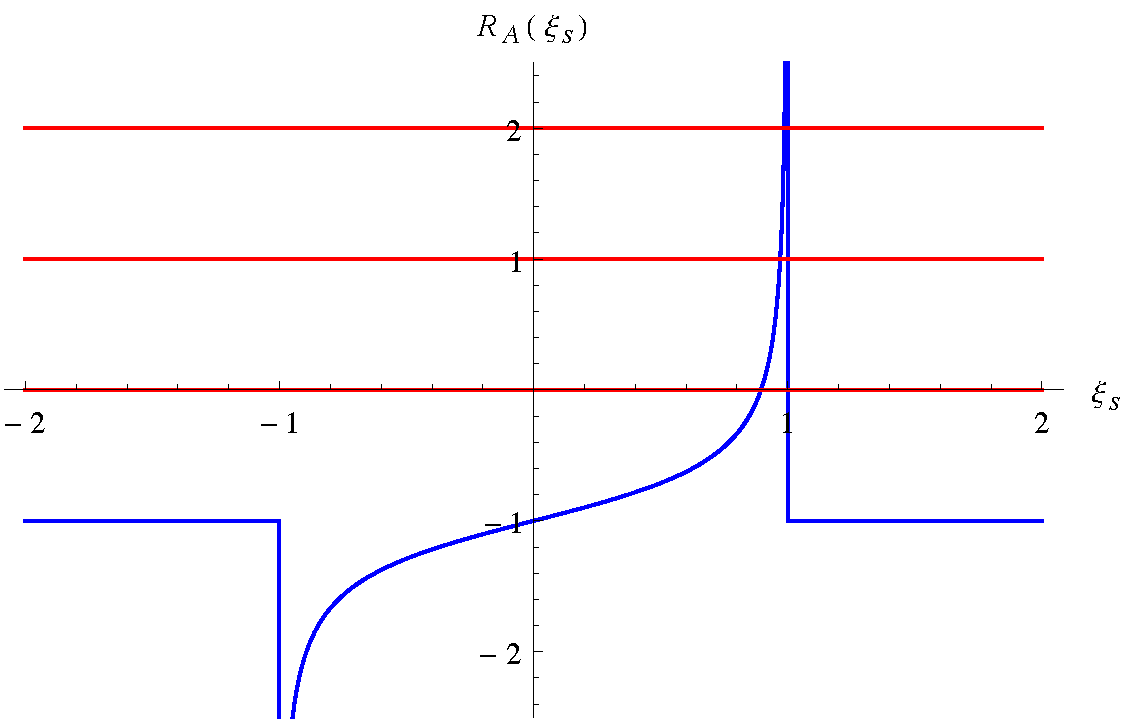
\includegraphics[scale=0.6]{Plots/ReRA.pdf}
\caption[Real part of the Regge trajectory function for the massless vector exchange model]{Real part of $R_{A}(\xi_{s})$. The red lines correspond to $R_{A} = 0, 1, 2$. We have used $Z_{a} Z_{b} \alpha_{1} = -0.5$.}
\label{ReRAFig}
\end{figure}

\begin{figure}
\centering
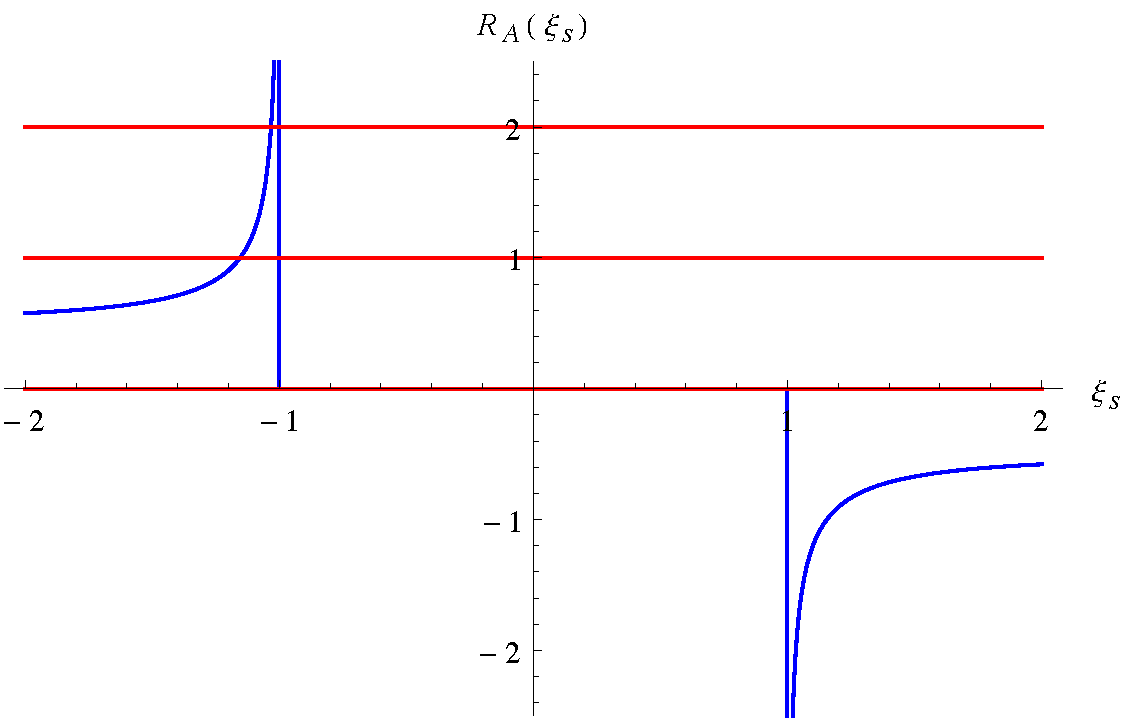
\includegraphics[scale=0.6]{Plots/ImRA.pdf}
\caption[Imaginary part of the Regge trajectory function for the massless vector exchange model]{Imaginary part of $R_{A}(\xi_{s})$. The red lines correspond to $R_{A} = 0, 1, 2$. We have used $Z_{a} Z_{b} \alpha_{1} = -0.5$.}
\label{ImRAFig}
\end{figure}